\documentclass[../1-Grundlagenteil.tex]{subfiles}
\begin{document}

\subsubsection*{Termschema von $^{87}$Rb}
    Rubidium $^{87}$Rb hat Zustände mit eine Hauptquantenzahl $n\in\{1,2,...,5\}$, wobei für $n=5$ nur ein Elektron vorhanden. Für Wechselwirkung mit diesen Schalenelektron ist der Gesamtspin also $S=1/2$. Grafik \ref{fig:Rb87Termschema} zeigt die ersten drei Energieniveaus für $n=5$.

    \begin{figure}[H]
        \centering
        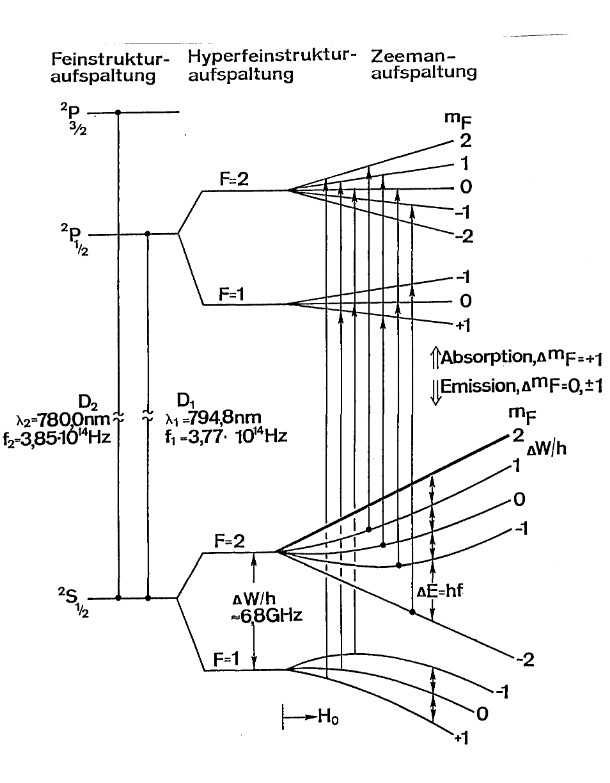
\includegraphics[width=8cm]{../../Bilddateien/Grundlagen/Rb87Termschema.jpg}
        \caption{Energieniveaus $^2\text{S}_{1/2}$, $^2\text{P}_{1/2}$ und $^2\text{P}_{3/2}$ von $^{87}$Rb und deren (Hyper-)Feinstrukturaufspaltung, sowie deren Zeeman-Aufspaltung \cite[p.171]{Schneider}}
        \label{fig:Rb87Termschema}
    \end{figure}

    Für diesen Versuch werden nur Übergänge zwischen Niveaus im Grundzustand betrachtet, für die $L=0$ gilt. Der Gesamtdrehimpuls ist also $J=L+S=S=1/2$.Daraus lassen sich die Landé-Faktoren der Quantenzahlen $J,F$ nun berechnen: es gilt
    \begin{align*}
        g_J &\approx 1 + \frac{J\cdot(J + 1) - L\cdot(L + 1) + S\cdot (S + 1)}{2\cdot J\cdot (J + 1)}
    \end{align*}
    und 
    \begin{align*}
        g_F &= g_J\cdot \frac{F\cdot(F + 1) + J\cdot(J + 1) - I\cdot (I + 1)}{2\cdot F\cdot (F + 1)}
    \end{align*}
    Einsetzen der gegebenen Werte liefert $g_J \approx 2$. Zum Vergleich: für reinen Bahnmagnetismus ($S=0$, also $L=J$) ist $g_J\approx 1$. Für reinen Spinmagnetismus ($L=2$) ist $g_S\approx 2$.\\

    \noindent Einsetzen von $g_J$, $F=I+J$ in die Formel für $g_F$ und umstellen nach $I$ liefert 
    \begin{align}
        I &= \frac{1}{g_F} - \frac{1}{2}
        \label{eq:KernspinFormel}
    \end{align} 

\subsubsection*{Optisches Pumpen}
    Wir betrachten der Einfachheit halber nur zwei Zustände: den Grundzustand G und den angeregten Zustand E. Diesen ordnen wir die Quantenzahlen $m_G,m_E\in\{-1/2,1/2}$ zu. Es ist nun ein äußeres $B$-Feld vorhanden und wir betrahlen das System mit $\sigma^+$-zirkular polarisierten Licht, welches parallel zu $B$ propagiert. Mit der Auswahlregel für $\sigma_+$ ergibt sich der Übergang $m_E = m_G + 1$. Dieser gehobene Zustand hat eine endliche Lebensdauer $\tau = 1 / \Gamma$, wobei $\Gamma$ die Übergangswahrscheinlichkeit pro Zeit repräsentiert. Nach dieser Dauer wird durch spontane Emission ein Grundzustand $m_G\in\{-1/2,1/2\}$ angestrebt. Die Wahrscheinlichkeit hierzu lässt sich mit Clebsch-Gordan-Koeffizienten beschreiben. Es gibt zwei Fälle: wenn $m_G=-1/2$, dann kann eine erneute Absorption eines $\sigma^+$-Photons stattfinden. Wenn jedoch $m_G=1/2$, so ist keine solche Absorption mehr möglich per Auswahlregel. Anschaulich gibt dieser Prozess das in Abbildung \ref{fig:OptischesPumpen} skizzierte Schema. 
    \begin{figure}[H]
        \centering
        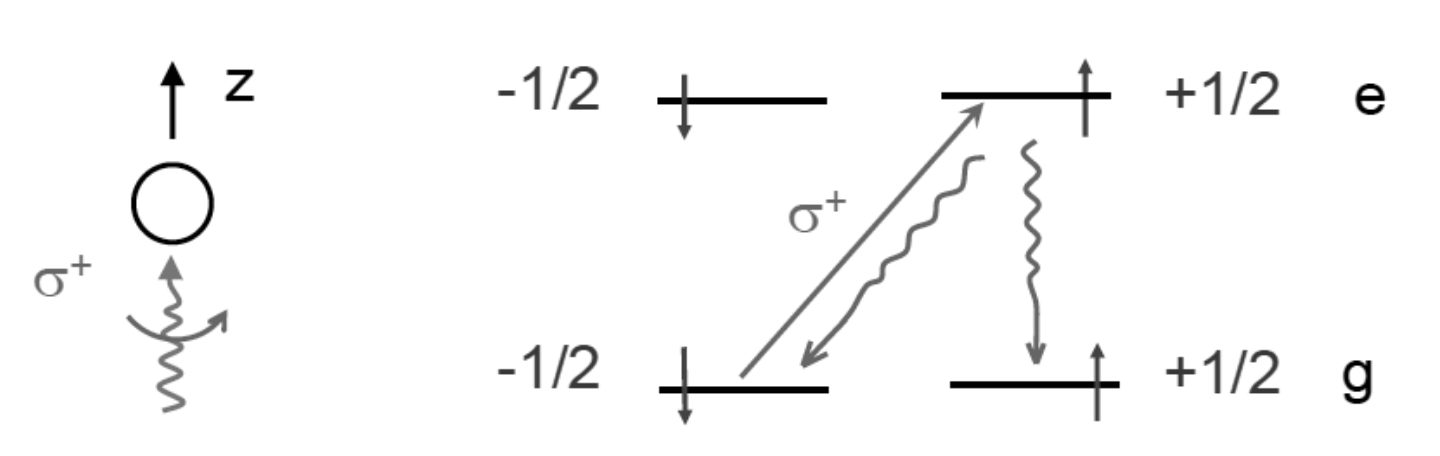
\includegraphics[width=9cm]{../../Bilddateien/Grundlagen/EasyQuantumPumping.png}
        \caption{Schematische Darstellung des optischen Pumpens.}
        \label{fig:OptischesPumpen}
    \end{figure}


    
\subsubsection*{Unterschiede zwischen $^{87}$Rb und $^{85}$Rb}
    Das Isotop $^{87}$Rb weißt den Kernspin $I_{87}=\frac{3}{2}$ auf, und $^{85}$Rb den Spin $I_{85}=\frac{5}{2}$. Diese unterschiedliche Kern-Bahn-Wechselwirkung sorgt zum einen für eine unterschiedlich starke Zeeman-Aufspaltung. Zum anderen sorgt die verschiedene Anzahl vorhandener Hyperfeinniveaus auch für eine verschiedene Anzahl von Zeeman-Niveaus \cite[180]{Schneider}.


\end{document}